\chapter{Comparative Experiments in the Lorenz 96 System}
\label{chap:lorenz96_experiments}

This chapter evaluates the performance of NFF in the Lorenz 96 system and compares it with PF and GPF. PF employs systematic resampling. Because particle degeneracy occurs easily in a 10-dimensional state space, the number of PF particles is increased to 5000, 10000, 30000, and 50000 to ensure filter stability. GPF uses the LCD-based deterministic sampling strategy, with particle counts of 2000, 5000, and 10000. For NFF, the particle counts are set to 500, 1000, and 2000. In the prediction step of NFF, Method 1 and Method 3 proposed in Chapter 3 are tested, and both the covariance-constrained (C) and unconstrained (NC) variants are evaluated.

The system is configured with state dimension $N=10$ and forcing parameter $F=8.0$. The discretization time step is set to $\Delta t=0.1$. All tests are conducted under the same initial uncertainty to ensure a fair comparison. To obtain statistically meaningful results, PF and GPF are evaluated over 20 independent Monte Carlo random seeds, whereas NFF is evaluated over 5 seeds. For each seed, the filtering process is run continuously for 100 time steps.

The source code for these experiments is available in \cite{Code_MA25_Wang}. This project relies on the libraries and implementations provided in \cite{Code_Filters_JL, Code_LCD_numeric, Code_DetGaussSampling}.

\section{Sensitivity to Noise Environments}
\label{sec:noise_sensitivity}

\subsection{Measurement Noise}
\label{subsec:measurement_noise}

This experiment evaluates the performance of different filters under different observation precisions. The intensity of the system process noise is fixed at 1, which, after discretization, corresponds to a cumulative process noise per step following a Gaussian distribution with variance 0.1. The control variable is the measurement noise variance, which is set to the sequence [0.01, 0.05, 0.1, 0.5, 1.0, 3.0].

In terms of state estimation accuracy, the RMSE and GAE curves in \Fig{fig:noise_rmse_gae} show that NFF achieves significantly higher accuracy than PF and GPF when the measurement noise is very small (e.g., 0.01). However, as the measurement noise gradually increases and the highly informative observations become less precise, the accuracy curves of NFF, PF, and GPF begin to converge and eventually exhibit similar performance.

\begin{Figure}[ht]
	\centering
	\begin{SubFigure}{\textwidth}
		\centering
		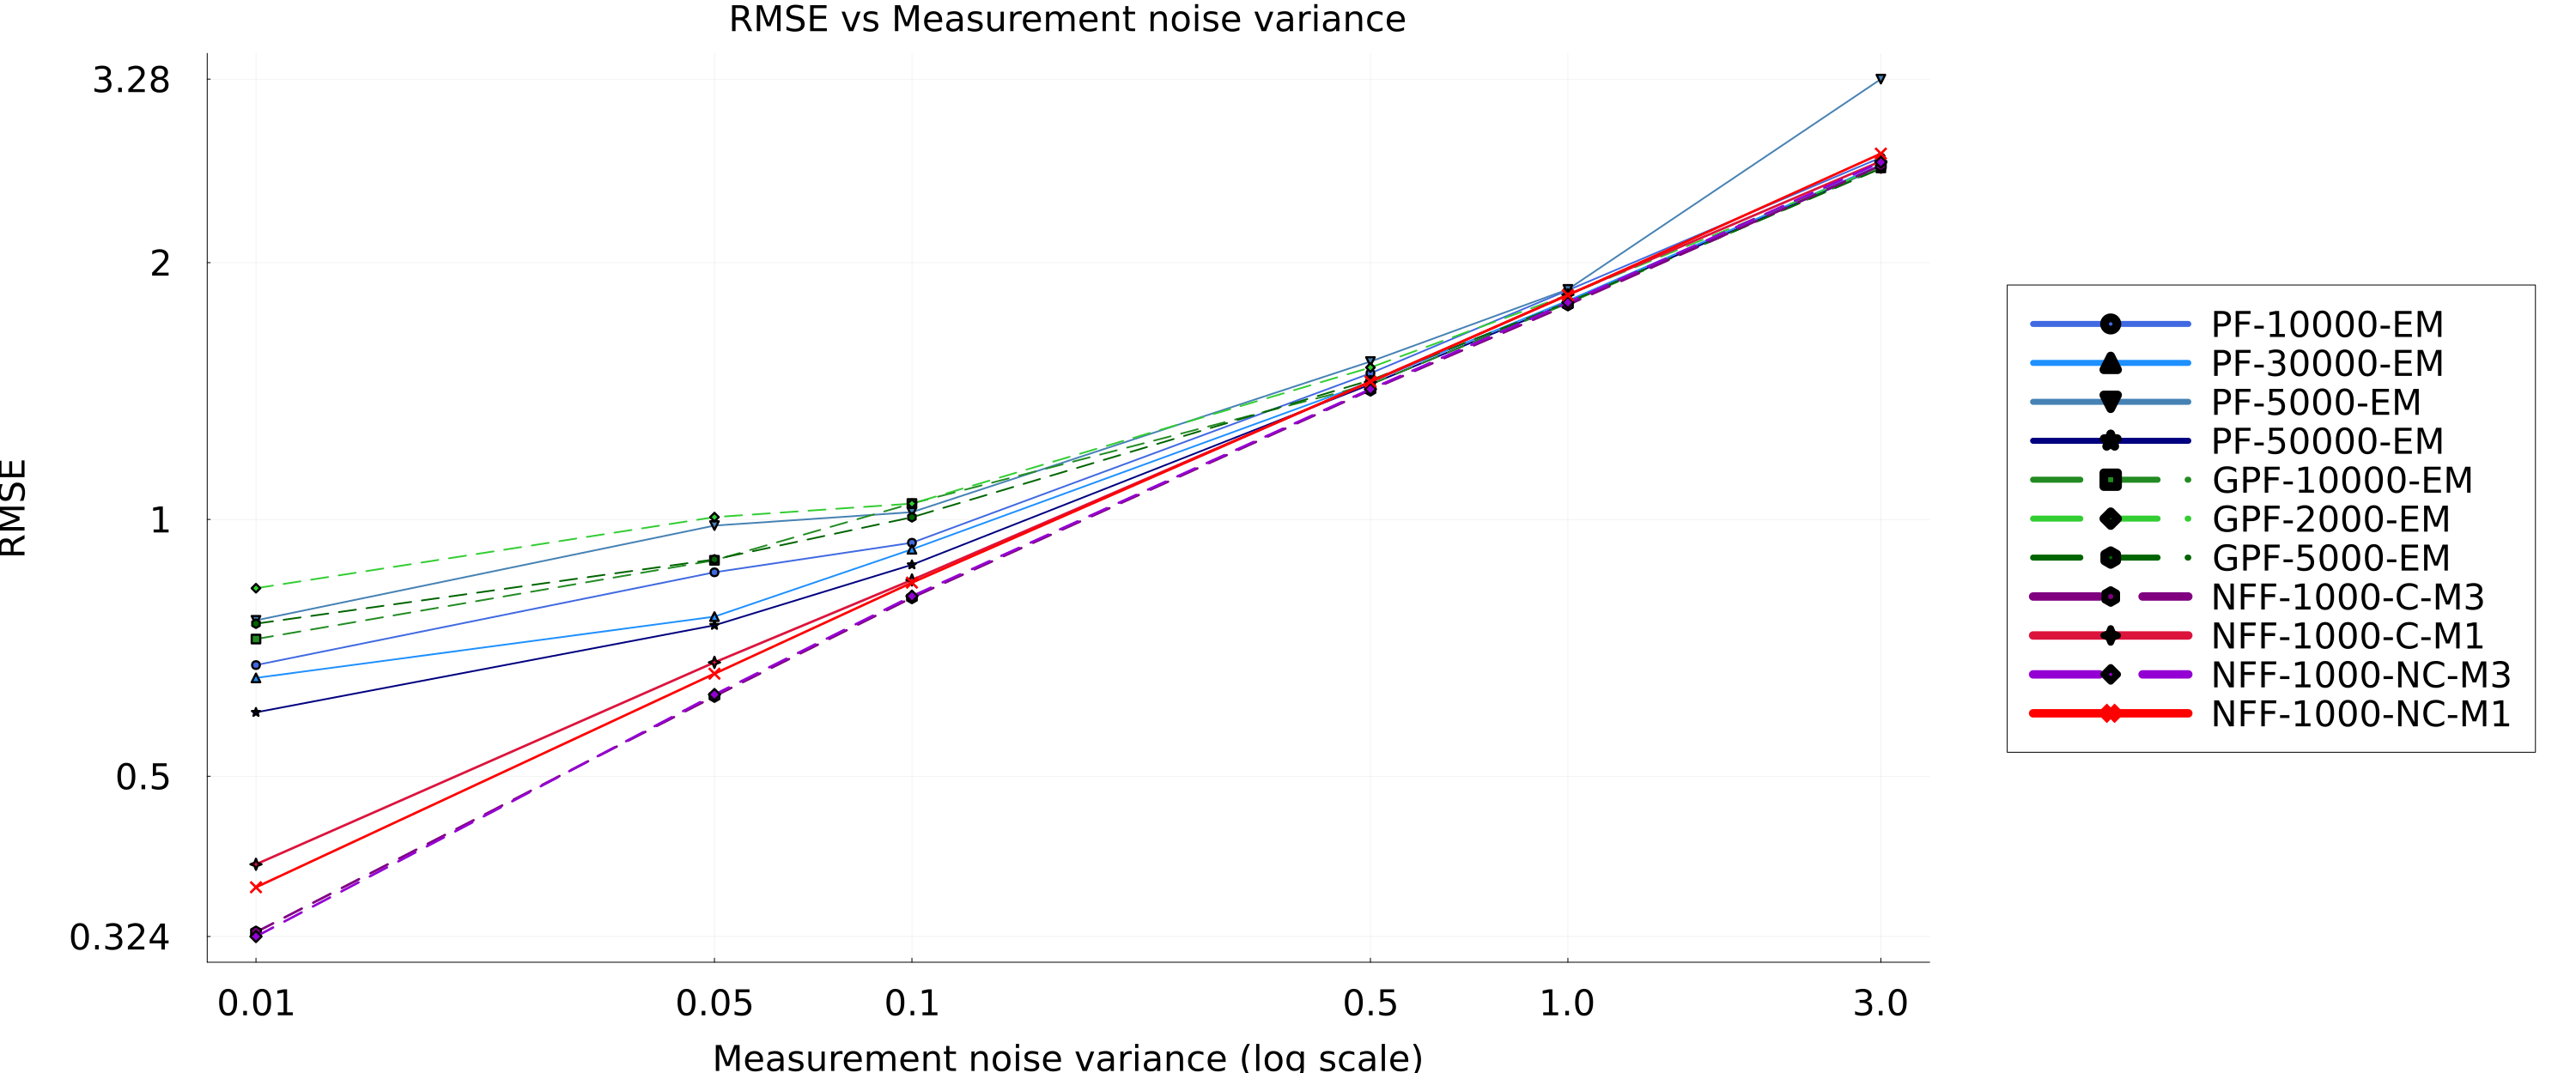
\includegraphics[width=\textwidth]{figures/Experiment06/rmse_nff_N1000_vs_others_rmse.png}
		\caption{RMSE vs. measurement noise variance.}
		\label{fig:noise_rmse}
	\end{SubFigure}
	
	\vspace{1.5em}
	
	\begin{SubFigure}{\textwidth}
		\centering
		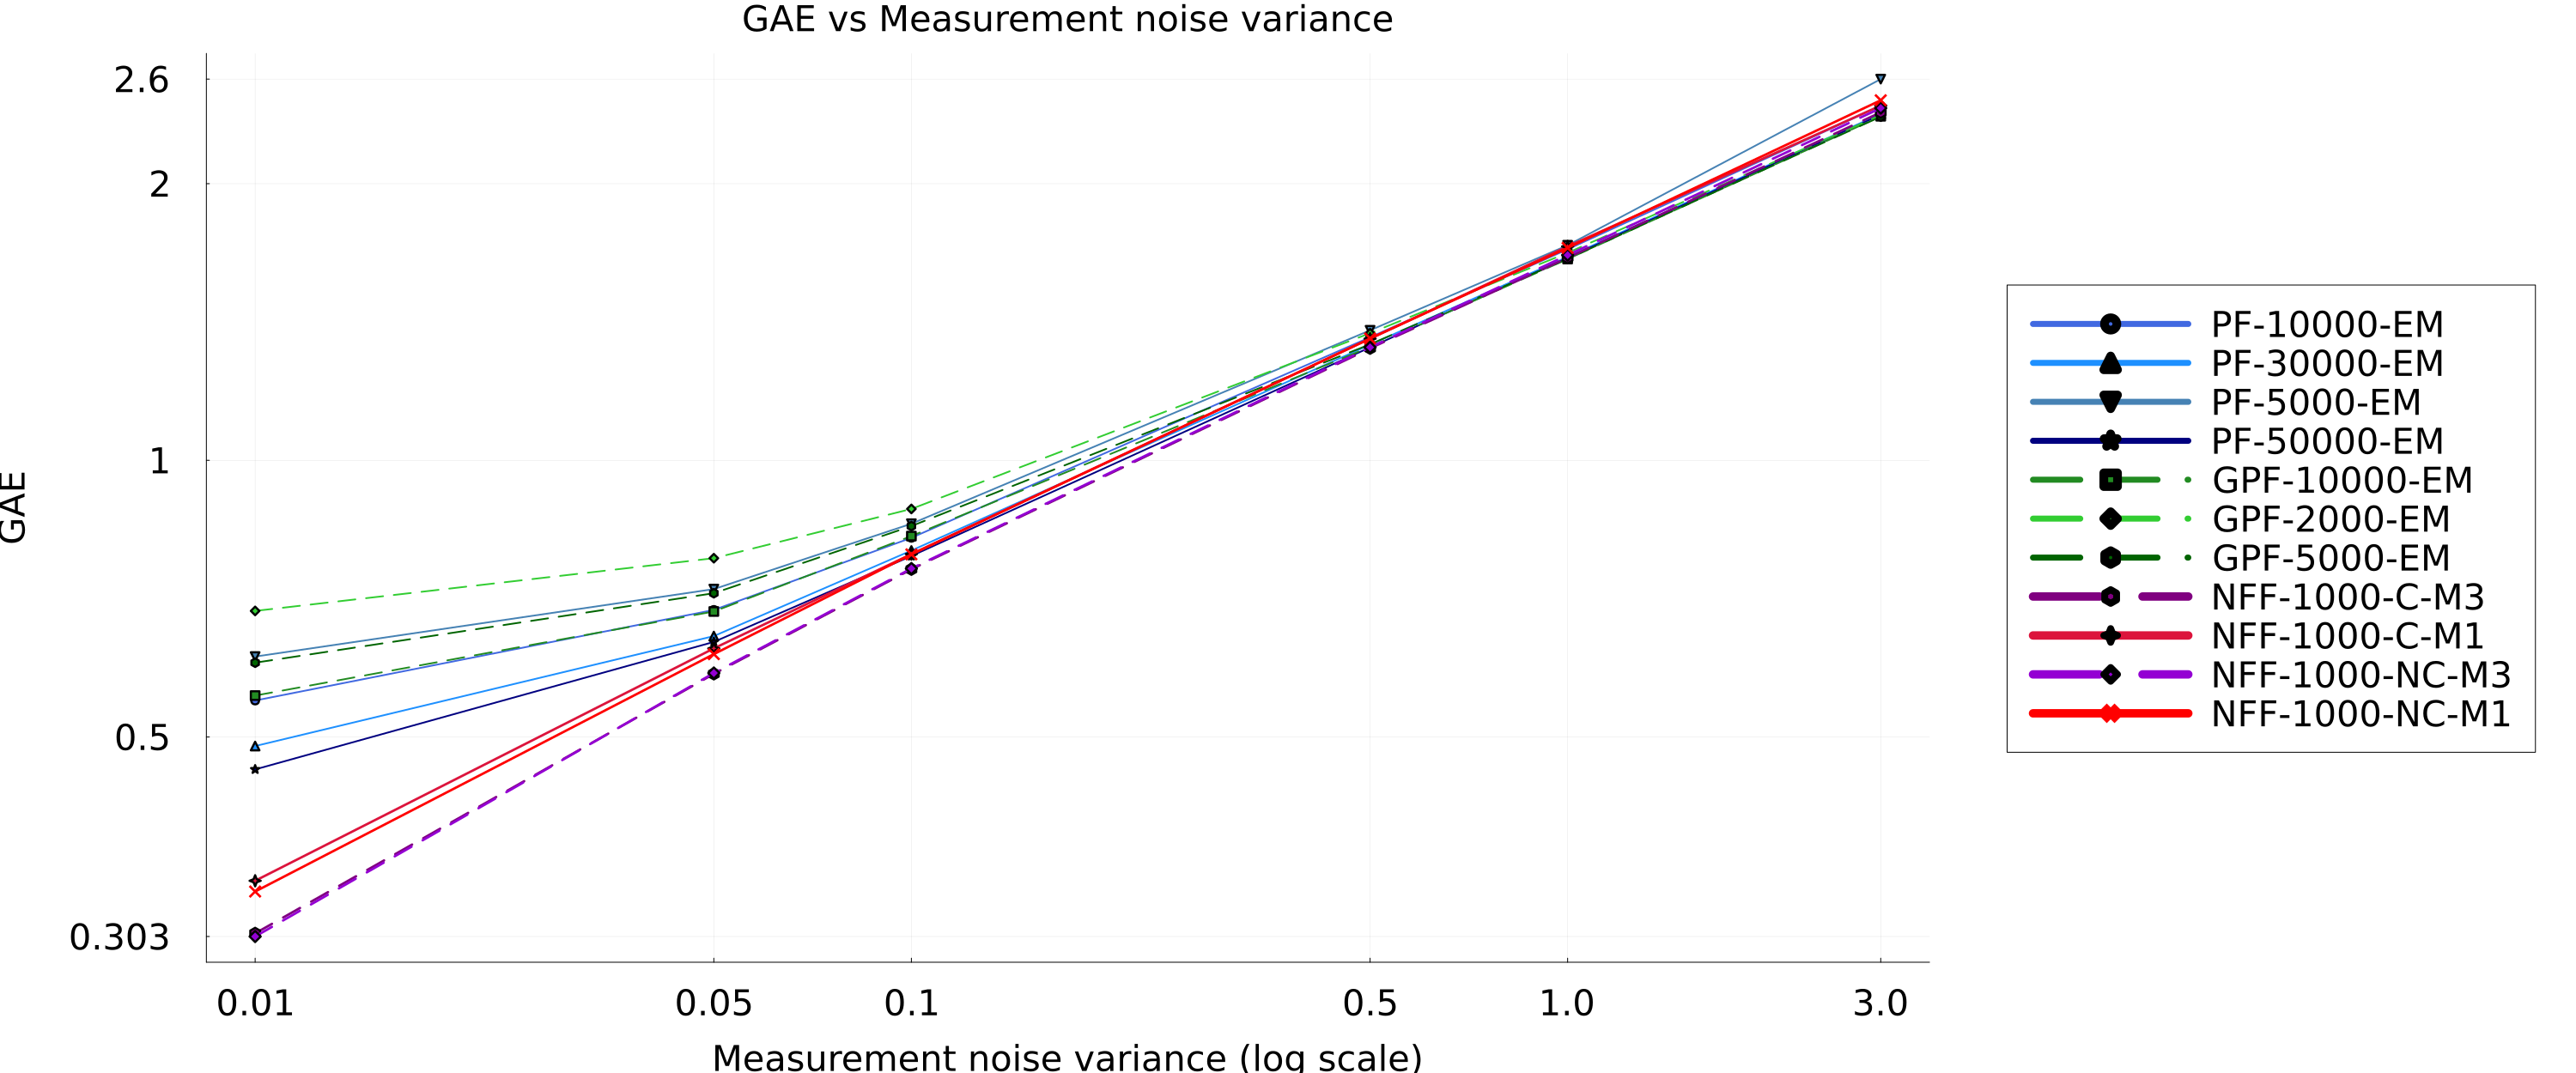
\includegraphics[width=\textwidth]{figures/Experiment06/gae_nff_N1000_vs_others_gae.png}
		\caption{GAE vs. measurement noise variance.}
		\label{fig:noise_gae}
	\end{SubFigure}
	\caption{RMSE and GAE vs. measurement noise variance.}
	\label{fig:noise_rmse_gae}
\end{Figure}

MERF reflects whether a filter effectively suppresses observation noise. Theoretically, in an ideal linear Gaussian setting with measurement noise variance 0.01 and prior cumulative system noise variance 0.1, the fused posterior noise variance is approximately $(0.1^{-1} + 0.01^{-1})^{-1} = 0.00909$. The corresponding ideal MERF value is $0.00909 / 0.01 = 0.909$. This indicates that when the sensor is already highly accurate, the theoretical room for further noise reduction by the filter is very limited.

In practical high-dimensional nonlinear systems, discretization error and particle approximation error make this ideal MERF almost unattainable. The experimental results in \Fig{fig:noise_merf} show that NFF with the third prediction mechanism maintains a MERF very close to 1.0. This means that it preserves the quality of the highly accurate observations without introducing substantial additional error. In contrast, PF with 50000 particles amplifies the original error by a factor of 1.87 after filtering, while GPF with 10000 particles amplifies it by more than a factor of 2. In the measurement-noise range from 0.05 to 0.1, the noise-suppression capability of NFF remains superior to that of PF and GPF. Only when the measurement noise increases further do the MERF values of all three filters converge.

\begin{Figure}[ht]
	\centering
	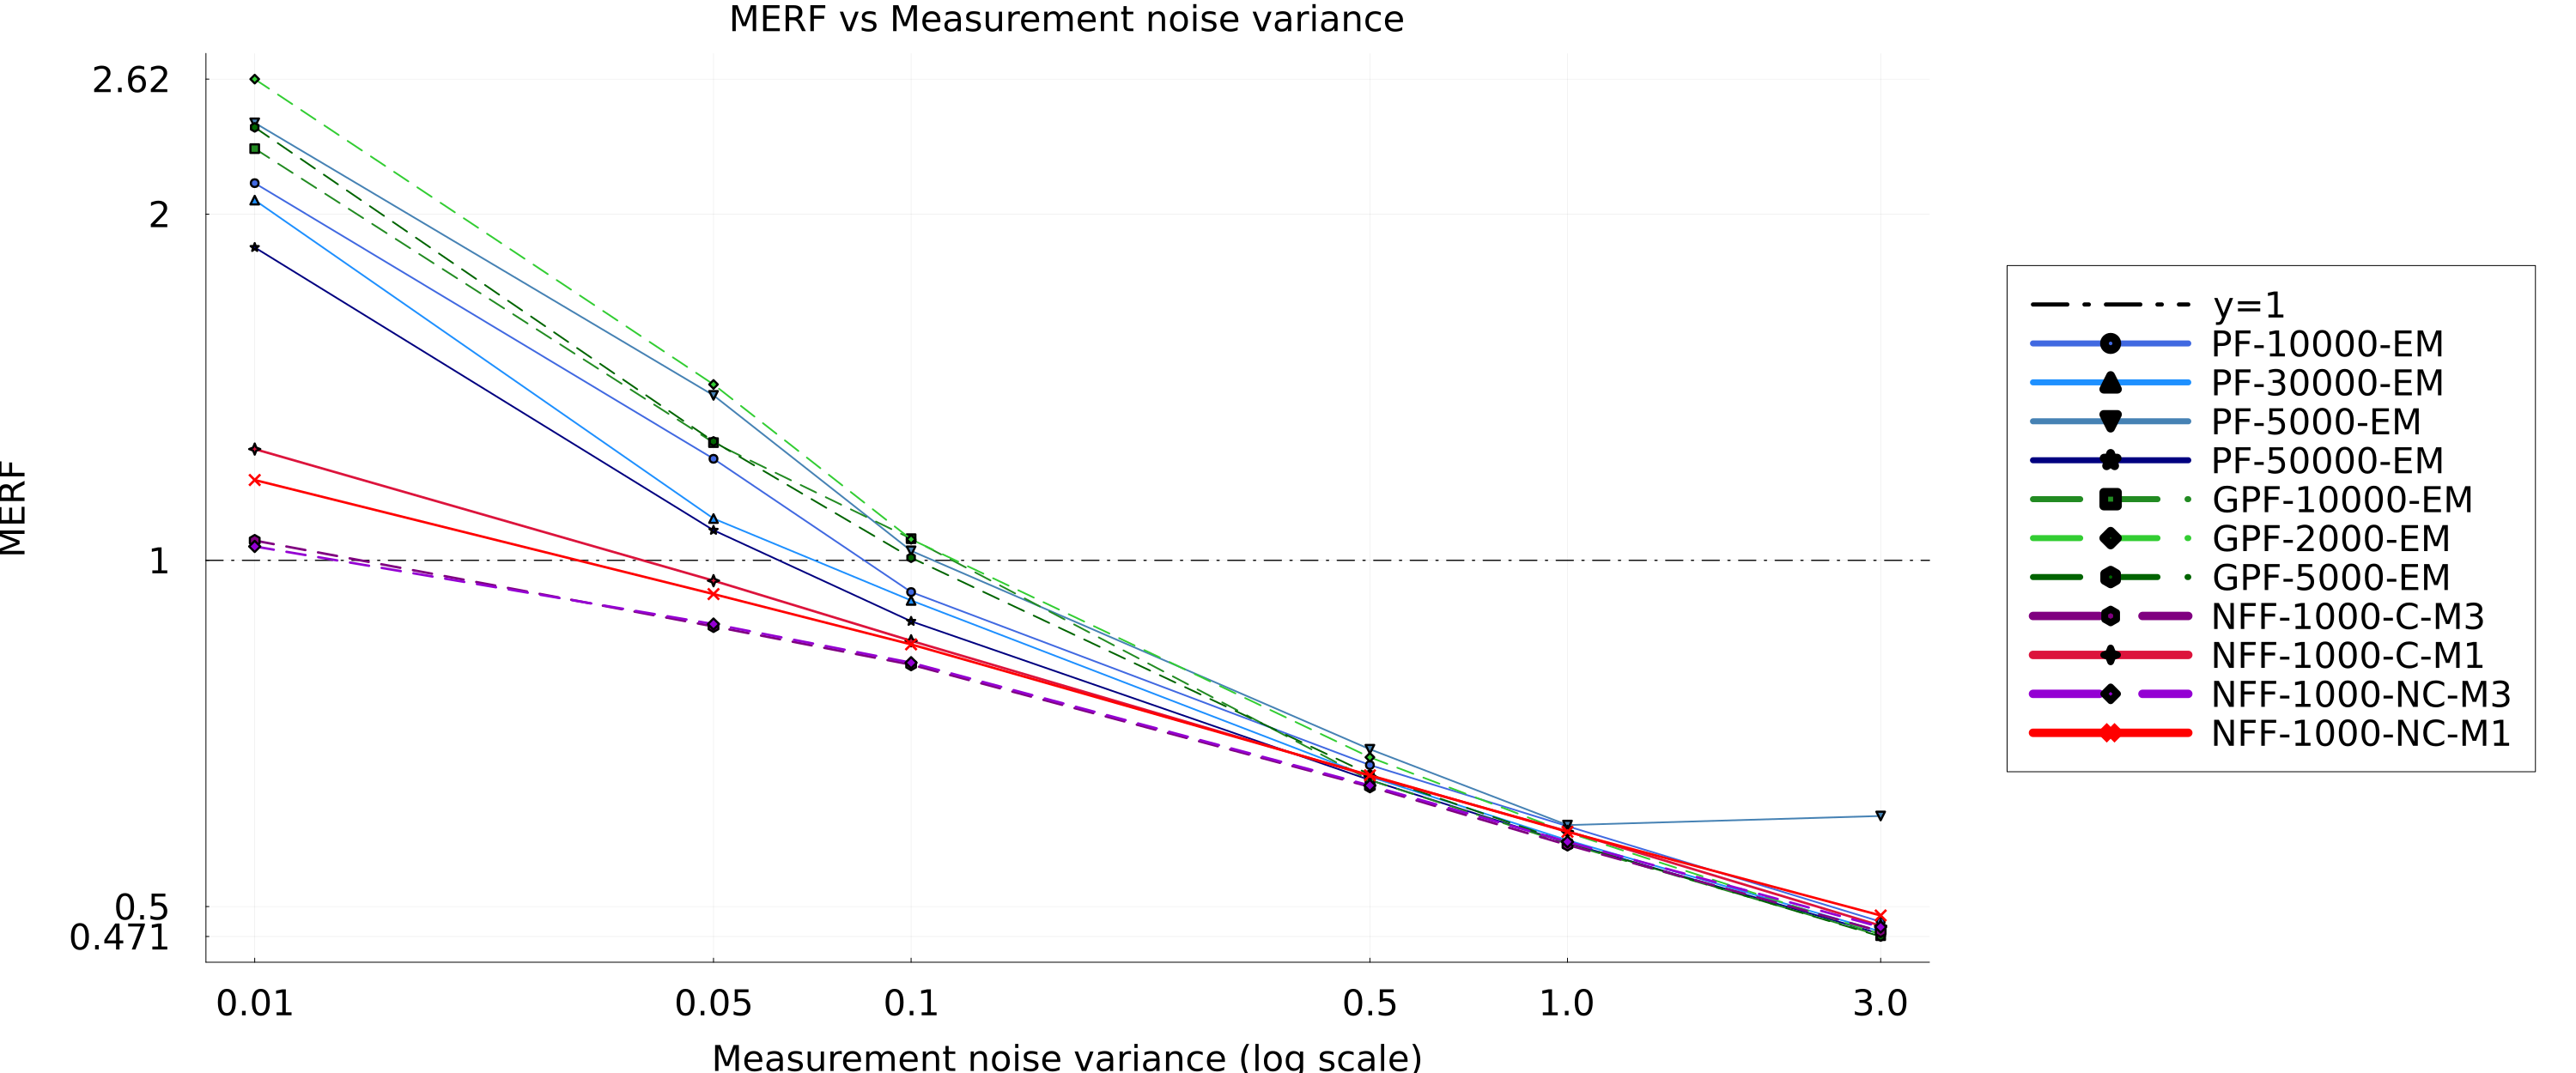
\includegraphics[width=\textwidth]{figures/Experiment06/merf_nff_N1000_vs_others_merf.png}
	\caption{MERF vs. measurement noise variance.}
	\label{fig:noise_merf}
\end{Figure}

ANEES is used to assess whether the filter becomes overconfident. As shown in \Fig{fig:noise_anees}, NFF with the third prediction mechanism behaves very stably, with ANEES consistently remaining below 2. This indicates that even under extremely narrow observation likelihoods, NFF maintains a sufficiently dispersed particle structure and that its estimated covariance reflects the actual estimation error reasonably well.

By contrast, for PF and GPF, when the measurement noise is extremely small (0.01 to 0.1), the narrow likelihood in the high-dimensional space causes severe particle degeneracy and sample impoverishment. The ANEES values of these two filters far exceed 100 and are therefore not visible in the plot because of the plotting scale. This implies that the particle sets of PF and GPF contract excessively and may even collapse to a single point, leading to severe overconfidence. Only when the measurement noise increases and the likelihood broadens do the ANEES values of PF and GPF return to normal levels and become comparable to those of NFF.

\begin{Figure}[ht]
	\centering
	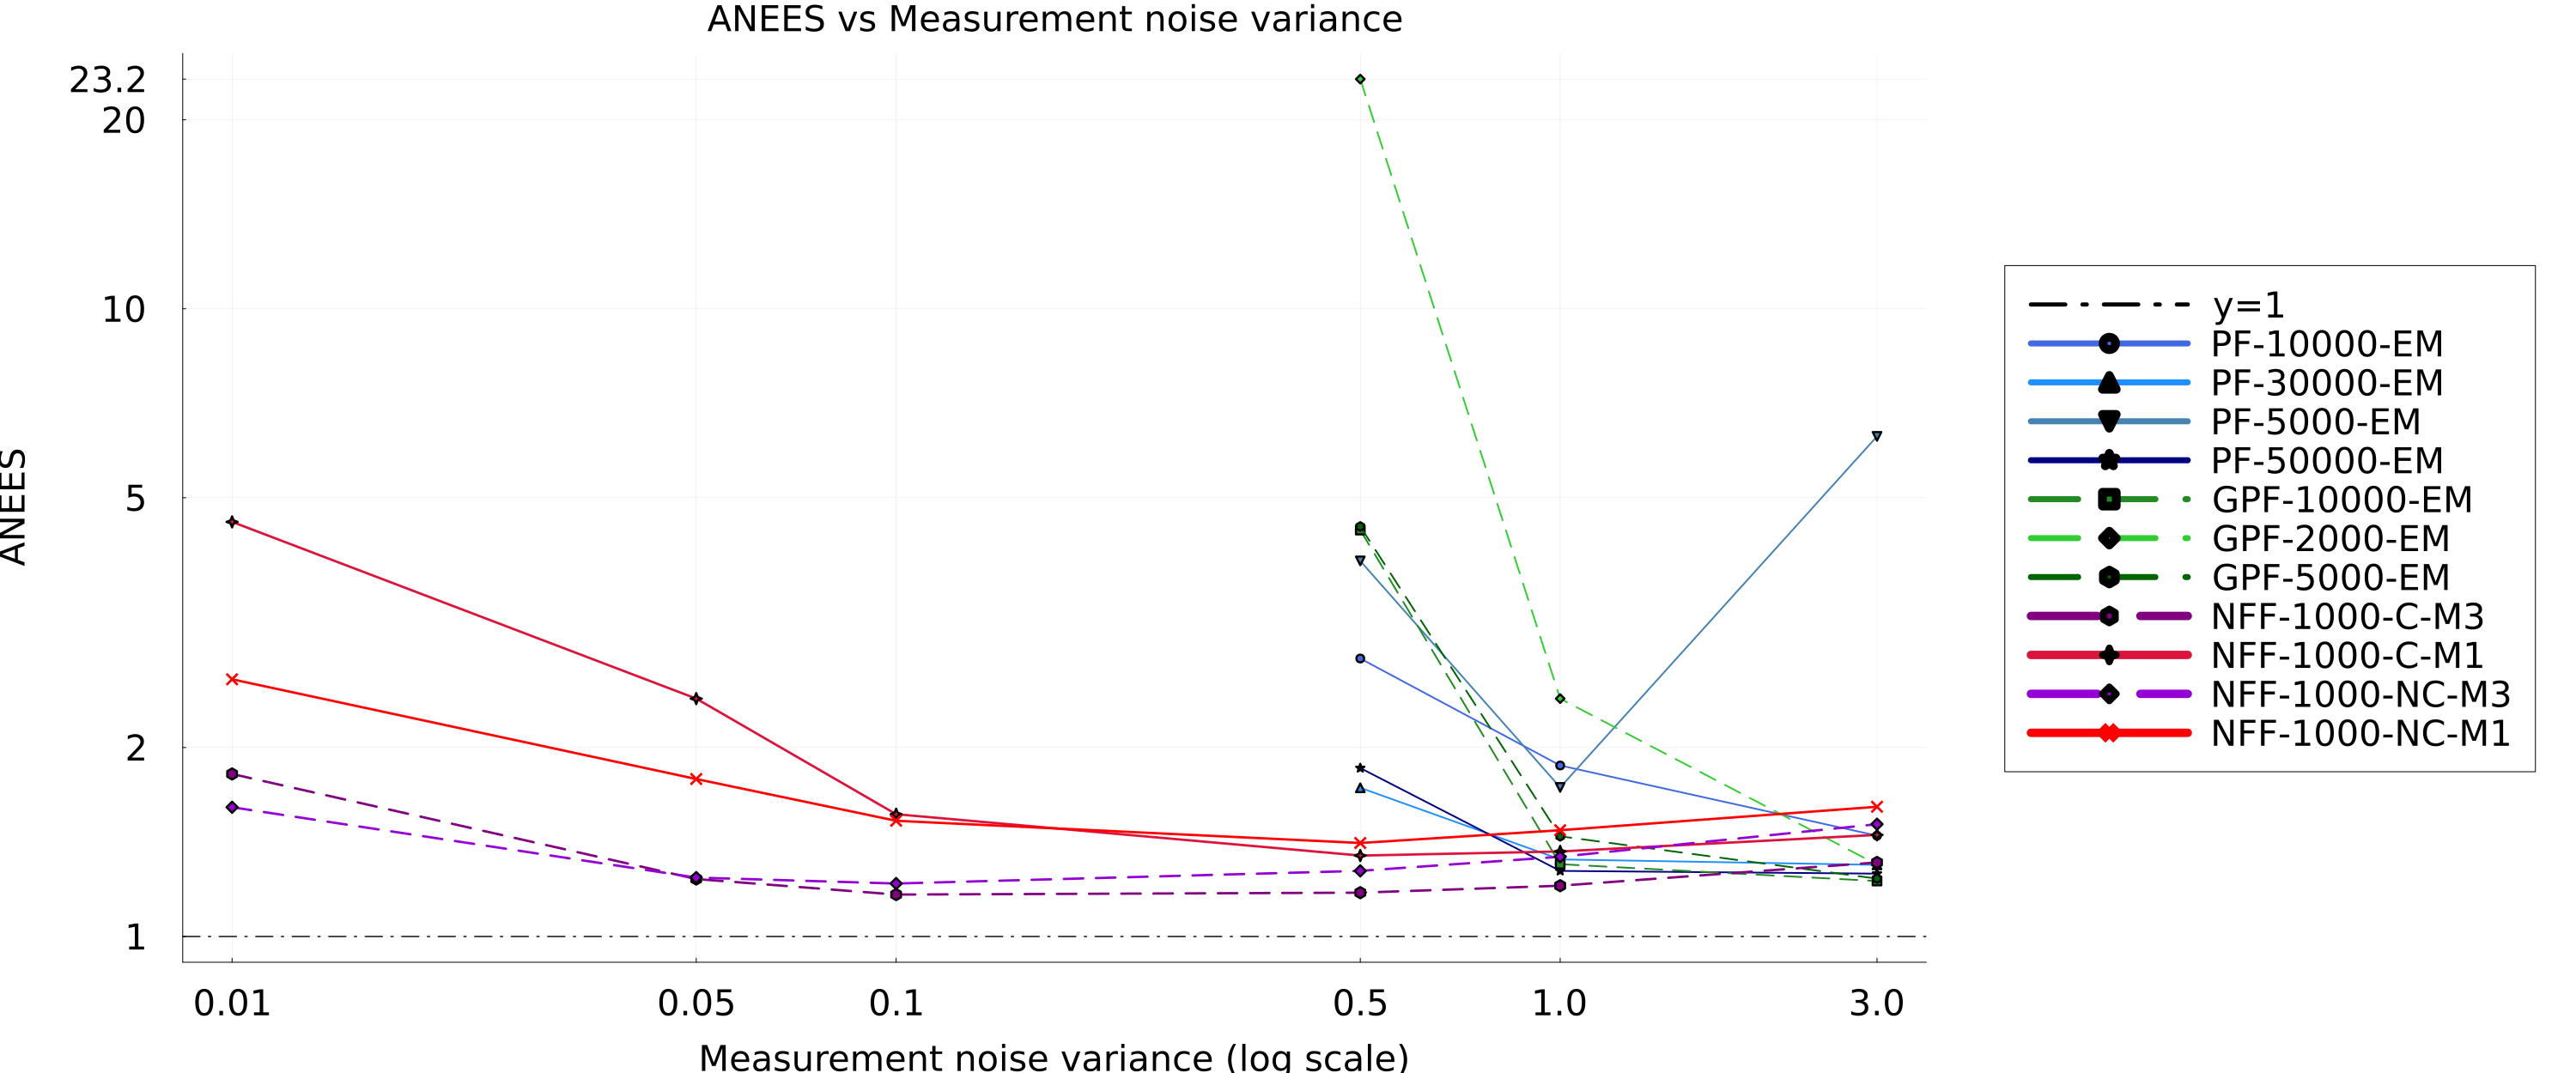
\includegraphics[width=\textwidth]{figures/Experiment06/anees_nff_N1000_vs_others_anees.png}
	\caption{ANEES vs. measurement noise variance.}
	\label{fig:noise_anees}
\end{Figure}

Taken together, these results show that in high-precision observation environments, traditional particle filters are highly susceptible to particle collapse and error amplification. In contrast, NFF effectively preserves particle diversity and exhibits a clear advantage in such scenarios.

\clearpage

\subsection{System Process Noise}
\label{subsec:system_noise}

This experiment evaluates the performance of different filters under different levels of system process noise. The measurement noise variance is fixed at 0.5. The control variable is the intensity of the system process noise, which is set to the sequence [0.1, 0.5, 1.0, 5.0, 10.0, 20.0]. After discretization, this corresponds to cumulative process noise variances per step of [0.01, 0.05, 0.1, 0.5, 1.0, 2.0].

In terms of state estimation accuracy, the RMSE and GAE curves in \Fig{fig:sysnoise_rmse_gae} show that the errors of all filters increase as the system process noise becomes larger. However, the accuracy curves of NFF gradually separate from those of PF and GPF. When the system noise is small (e.g., 0.1 and 0.5), the estimation accuracies of NFF, PF, and GPF are relatively similar. As the system noise continues to increase, the error growth of NFF remains noticeably slower, and the performance gap between NFF and the other two filters widens progressively.

\begin{Figure}[ht]
	\centering
	\begin{SubFigure}{\textwidth}
		\centering
		
\includegraphics[width=\textwidth]{figures/Experiment07/rmse_nff_N1000_vs_others_rmse.png}
		\caption{RMSE vs. system noise variance.}
		\label{fig:sysnoise_rmse}
	\end{SubFigure}
	
	\vspace{1.5em}
	
	\begin{SubFigure}{\textwidth}
		\centering
		
\includegraphics[width=\textwidth]{figures/Experiment07/gae_nff_N1000_vs_others_gae.png}
		\caption{GAE vs. system noise variance.}
		\label{fig:sysnoise_gae}
	\end{SubFigure}
	\caption{RMSE and GAE vs. system noise variance.}
	\label{fig:sysnoise_rmse_gae}
\end{Figure}

The MERF results further emphasize the advantage of NFF. The data in \Fig{fig:sysnoise_merf} shows that the larger the system noise becomes, the better NFF performs relative to PF and GPF in suppressing observation noise. Under extreme high-interference conditions, where the system process noise intensity reaches 20.0, the MERF of NFF remains below 1.0 (approximately 0.8), meaning that effective noise reduction is still achieved. In contrast, under the same conditions, the MERF values of PF and GPF are far above 1.0, indicating that their filtering updates actually amplify the original measurement error substantially.

\begin{Figure}[ht]
	\centering
	
\includegraphics[width=\textwidth]{figures/Experiment07/merf_nff_N1000_vs_others_merf.png}
	\caption{MERF vs. system noise variance.}
	\label{fig:sysnoise_merf}
\end{Figure}

In terms of ANEES, NFF shows excellent robustness. As illustrated in \Fig{fig:sysnoise_anees}, its ANEES remains below 2 across all tested system noise levels and stays very close to 1 when the system noise is extremely large. This indicates that NFF maintains a realistic assessment of its estimation uncertainty while preserving a reasonable particle structure. By contrast, PF and GPF can maintain a somewhat dispersed particle structure only when the system noise is small. As the system noise increases, the ANEES values of PF and GPF rise rapidly and exceed 100, again truncated in the plot because of the scale. This indicates that under high system noise, the particle sets of PF and GPF undergo severe over-contraction and may collapse to a single point, causing the covariance estimate to fail completely and the filters to become extremely overconfident.

\begin{Figure}[ht]
	\centering
	
\includegraphics[width=\textwidth]{figures/Experiment07/anees_nff_N1000_vs_others_anees.png}
	\caption{ANEES vs. system noise variance.}
	\label{fig:sysnoise_anees}
\end{Figure}

Overall, these results indicate that NFF is better suited to high-dimensional complex systems with large process noise and is more capable of extracting useful information from highly noisy environments to reduce observation error.

The underlying reason is the difference in how the prior information is utilized. When the system process noise is very large, the prior particle set generated by the prediction step becomes highly dispersed and sparse in the state space. For PF and GPF, only a very small number of particles fall within the effective support of the likelihood, while the vast majority are effectively discarded after the weight update. As a result, most of the prior information generated by the system dynamics is wasted. By contrast, NFF uses a homotopy mechanism to drive the dispersed prior particles smoothly toward the posterior region, thereby making much more effective use of the prior information.
\clearpage

\section{Sensitivity to System Nonlinearity Intensity}
\label{sec:nonlinearity_sensitivity}

This experiment evaluates the filtering performance under different levels of system nonlinearity. The system process noise is fixed at 1, and the measurement noise variance is fixed at 0.5. The control variable is the discretization time step $\Delta t$, which is set to the sequence [0.01, 0.1, 0.15, 0.4, 0.6]. In a nonlinear system, a larger integration step $\Delta t$ implies stronger nonlinearity within a single propagation step, making the system evolution increasingly difficult to predict.

In terms of state estimation accuracy, the RMSE and GAE curves in \Fig{fig:nonlinear_rmse_gae} show that the errors of all filters increase as the discretization step $\Delta t$ becomes larger and the state evolution becomes harder to predict. When $\Delta t$ is small (0.01 to 0.15), the accuracy of NFF is comparable to that of PF and GPF. However, as the step size increases further to 0.4 and 0.6, the accuracy curves of NFF begin to separate from those of PF and GPF. The error growth of NFF is noticeably smaller, indicating better estimation capability under strongly nonlinear conditions.

\begin{Figure}[ht]
	\centering
	\begin{SubFigure}{\textwidth}
		\centering
		
\includegraphics[width=\textwidth]{figures/Experiment08/rmse_nff_N1000_vs_others_rmse.png}
		\caption{RMSE vs. discretization time step.}
		\label{fig:nonlinear_rmse}
	\end{SubFigure}
	
	\vspace{1.5em}
	
	\begin{SubFigure}{\textwidth}
		\centering
		
\includegraphics[width=\textwidth]{figures/Experiment08/gae_nff_N1000_vs_others_gae.png}
		\caption{GAE vs. discretization time step.}
		\label{fig:nonlinear_gae}
	\end{SubFigure}
	\caption{RMSE and GAE vs. discretization time step.}
	\label{fig:nonlinear_rmse_gae}
\end{Figure}

MERF clearly reflects the noise-rejection performance of the filters under strong model nonlinearity. As shown in \Fig{fig:nonlinear_merf}, when $\Delta t$ lies between 0.01 and 0.15, the performance gap among the filters is relatively small. A clear turning point appears at $\Delta t = 0.4$. At this point, the system nonlinearity is already very strong, and the update steps of PF and GPF actually amplify the measurement noise, with MERF far above 1. By contrast, NFF still reduces the observation noise effectively.

However, when the step size is increased further to the extreme value $\Delta t = 0.6$, the large time interval makes the prediction step highly inaccurate. At this stage, the prediction step provides little useful prior information for the update and may even provide misleading information. Under this extreme condition, where the prediction model itself essentially fails, the MERF values of NFF, PF, and GPF all deteriorate severely.

\begin{Figure}[ht]
	\centering
	
\includegraphics[width=\textwidth]{figures/Experiment08/merf_nff_N1000_vs_others_merf.png}
	\caption{MERF vs. discretization time step.}
	\label{fig:nonlinear_merf}
\end{Figure}

The ANEES results in \Fig{fig:nonlinear_anees} further support this interpretation. When $\Delta t$ is small (0.01 to 0.1), PF, GPF, and NFF all maintain a reasonable particle structure and do not show obvious overconfidence. However, when $\Delta t$ increases to 0.4 and 0.6, the ANEES values of PF and GPF exceed 100, indicating that under strong nonlinear mappings their particle sets again suffer severe degeneracy and collapse.

It is worth noting that NFF also exhibits overconfidence when $\Delta t$ is large, as reflected by its significantly increased ANEES value. This is not caused by particle collapse in NFF, but rather by the fact that the overly large time interval makes the predicted prior positions highly inaccurate. This large prediction bias then affects the final update result, producing a larger actual estimation error.

\begin{Figure}[ht]
	\centering
	
\includegraphics[width=\textwidth]{figures/Experiment08/anees_nff_N1000_vs_others_anees.png}
	\caption{ANEES vs. discretization time step.}
	\label{fig:nonlinear_anees}
\end{Figure}

Taken together, these results suggest that NFF is well suited to strongly nonlinear scenarios in which prediction is difficult. As long as the state evolution equation can still provide at least a small amount of useful prior information, NFF is much more capable than PF and GPF of exploiting this weak information to suppress observation noise. However, if the nonlinearity becomes so strong that the prediction model fails completely and no longer provides valid prior information, NFF also suffers unavoidable performance degradation.

\clearpage

\section{Sensitivity to Model Mismatch}
\label{sec:mismatch_sensitivity}

To evaluate the performance of each filter under non-ideal conditions, this experiment introduces model mismatch artificially. Perturbations of $\pm 20\%$ are applied to the system process noise covariance matrix $Q$, the measurement noise covariance matrix $R$, the state model $f(x)$, and the observation model $h(x)$ in order to assess the robustness of the algorithms.

When perturbations are applied to the noise parameters (overestimated or underestimated $Q$ and $R$) and the observation model (overestimated or underestimated $h(x)$), the results show that NFF with 1000 particles performs comparably to the best PF configuration with up to 50000 particles and the best GPF configuration with 10000 particles. As reported in \Tab{tab:full_mismatch_results_v2}, the differences in three of the four error metrics (RMSE, GAE, and MERF) remain comparable, whereas NFF outperforms PF and GPF in ANEES. This indicates that while all three filters maintain basic robustness to moderate mismatches, NFF estimates its own uncertainty more accurately.

However, when a $+20\%$ mismatch is introduced into the system model $f(x)$, NFF exhibits a clear advantage in estimation accuracy. Compared with the best PF and GPF results, its RMSE is reduced by about $18\%$--$29\%$, while its MERF is improved by approximately $17\%$--$28\%$. More importantly, in terms of ANEES, which reflects filter consistency, both PF and GPF collapse completely under this condition, with ANEES diverging to \textit{NaN}. In contrast, both variants of NFF (M1 and M3) remain stable and convergent, with ANEES staying within a clearly reasonable range.

The fundamental reason why NFF remains highly robust to mismatch in the system model is consistent with the mechanism discussed earlier. Even when the prediction is no longer sufficiently accurate, NFF can still exploit the prior information effectively.

\begin{Table}[ht]
	\caption{Performance under $\pm 20\%$ model mismatches. Comparison between the best PF/GPF and NFF ($L=1000$).}
	\label{tab:full_mismatch_results_v2}
	\footnotesize
	\setlength{\tabcolsep}{5pt}
	\begin{tabular}{|c|l|c|c|cc|cc|}
		\hline
		& & & & \multicolumn{2}{c|}{NFF (C)} & \multicolumn{2}{c|}{NFF (NC)} \\ \cline{5-8}
		Mismatch Type & Metric & Best PF & Best GPF & M3  & M1  & M3  & M1  \\ \hline
		
		{$+20\% Q$}
		& RMSE  & 1.459 & 1.469 & \textbf{1.409} & 1.439 & 1.410 & 1.444 \\
		& GAE   & 1.344 & 1.348 & \textbf{1.318} & 1.346 & 1.319 & 1.350 \\
		& MERF  & 0.653 & 0.657 & \textbf{0.631} & 0.645 & 0.632 & 0.647 \\
		& ANEES & 1.398 & 1.935 & \textbf{1.071} & 1.209 & 1.141 & 1.274 \\ \hline
		
		{$-20\% Q$}
		& RMSE  & 1.519 & 1.875 & \textbf{1.432} & 1.483 & 1.445 & 1.495 \\
		& GAE   & 1.385 & 1.397 & \textbf{1.338} & 1.386 & 1.346 & 1.396 \\
		& MERF  & 0.679 & 0.839 & \textbf{0.645} & 0.668 & 0.648 & 0.670 \\
		& ANEES & 1.785 & NaN   & \textbf{1.344} & 1.585 & 1.480 & 1.686 \\ \hline
		
		{$+20\% R$}
		& RMSE  & 1.484 & 1.484 & \textbf{1.459} & 1.479 & 1.464 & 1.499 \\
		& GAE   & \textbf{1.362} & \textbf{1.362} & 1.406 & 1.426 & 1.411 & 1.443 \\
		& MERF  & \textbf{0.664} & \textbf{0.664} & \textbf{0.664} & 0.673 & 0.666 & 0.682 \\
		& ANEES & 1.265 & 1.629 & \textbf{1.133} & 1.239 & 1.237 & 1.430 \\ \hline
		
		{$-20\% R$}
		& RMSE  & 1.479 & 1.490 & \textbf{1.432} & 1.451 & 1.435 & 1.461 \\
		& GAE   & \textbf{1.356} & 1.362 & 1.379 & 1.398 & 1.382 & 1.410 \\
		& MERF  & 0.662 & 0.667 & \textbf{0.652} & 0.660 & 0.653 & 0.665 \\
		& ANEES & 1.878 & 7.101 & \textbf{1.344} & 1.478 & 1.443 & 1.620 \\ \hline
		
		{$+20\% f(x)$}
		& RMSE  & 1.947 & 2.227 & \textbf{1.581} & 1.645 & 1.606 & 1.666 \\
		& GAE   & 1.550 & 1.575 & \textbf{1.534} & 1.602 & 1.559 & 1.616 \\
		& MERF  & 0.871 & 0.996 & \textbf{0.720} & 0.749 & 0.731 & 0.758 \\
		& ANEES & NaN   & NaN   & \textbf{1.508} & 1.846 & 1.720 & 2.050 \\ \hline
		
		{$-20\% f(x)$}
		& RMSE  & 1.666 & 1.668 & \textbf{1.578} & 1.657 & 1.607 & 1.681 \\
		& GAE   & 1.554 & 1.548 & \textbf{1.524} & 1.599 & 1.554 & 1.631 \\
		& MERF  & 0.745 & 0.746 & \textbf{0.718} & 0.754 & 0.731 & 0.765 \\
		& ANEES & 2.005 & 2.801 & \textbf{1.418} & 1.785 & 1.607 & 1.987 \\ \hline
		
		{$+20\% h(x)$}
		& RMSE  & 2.649 & 2.663 & 2.509 & 2.585 & \textbf{2.497} & 2.514 \\
		& GAE   & 2.528 & 2.534 & 2.452 & 2.528 & \textbf{2.440} & 2.453 \\
		& MERF  & 0.852 & 0.856 & 0.833 & 0.858 & \textbf{0.829} & 0.834 \\
		& ANEES & 9.071 & 24.620& \textbf{4.242} & 5.546 & 4.360 & 5.034 \\ \hline
		
		{$-20\% h(x)$}
		& RMSE  & 2.867 & 3.225 & 2.852 & 2.922 & \textbf{2.779} & 2.823 \\
		& GAE   & \textbf{2.681} & 2.777 & 2.799 & 2.874 & 2.731 & 2.775 \\
		& MERF  & 0.613 & 0.690 & 0.620 & 0.635 & \textbf{0.604} & 0.614 \\
		& ANEES & 14.986 & NaN  & \textbf{3.438} & 4.325 & 3.767 & 4.199 \\ \hline
	\end{tabular}
\end{Table}

\clearpage

\section{Extreme Condition Tests}
\label{sec:extreme_conditions}

This experiment considers four extreme combinations of system process noise $Q$ and observation noise $R$. Through these comparative tests, the advantages and applicable scenarios of NFF are clarified.

When the system is subject to both large system noise and large observation noise, prediction becomes difficult and the sensor measurements become highly unreliable. Under this severely adverse condition, all filters perform poorly, with errors increasing to very large values (all RMSE values approach 6.0). As shown in \Tab{tab:extreme_noise_v2}, the performance of NFF is not significantly different from that of PF and GPF.

When the system has small process noise but large observation noise, the likelihood function becomes broad and relatively flat in the state space. Under this condition, GPF achieves the best performance. NFF ranks second, but remains inferior to GPF.

In the scenario with small system noise and small observation noise, both the prior and the likelihood are highly concentrated. As a result, PF and GPF suffer from severe particle degeneracy, and their consistency metric (ANEES) collapses. NFF, by contrast, remains stable and reduces the RMSE by more than 20\% relative to PF and GPF.

In the scenario with large system noise and small observation noise, the results show that PF and GPF diverge completely. Not only do their ANEES values become NaN, but their filtering outputs also amplify the original measurement error by a factor of four to five, with MERF reaching 4.272 and 5.283, respectively. By contrast, NFF remains stable, improves the estimation accuracy by up to 70\%, and keeps MERF within a reasonable range.

A summary of the dominant performance regions for the different filters under these varied noise conditions is illustrated in \Fig{fig:noise_quadrant}.

\begin{Figure}[ht]
    \centering
    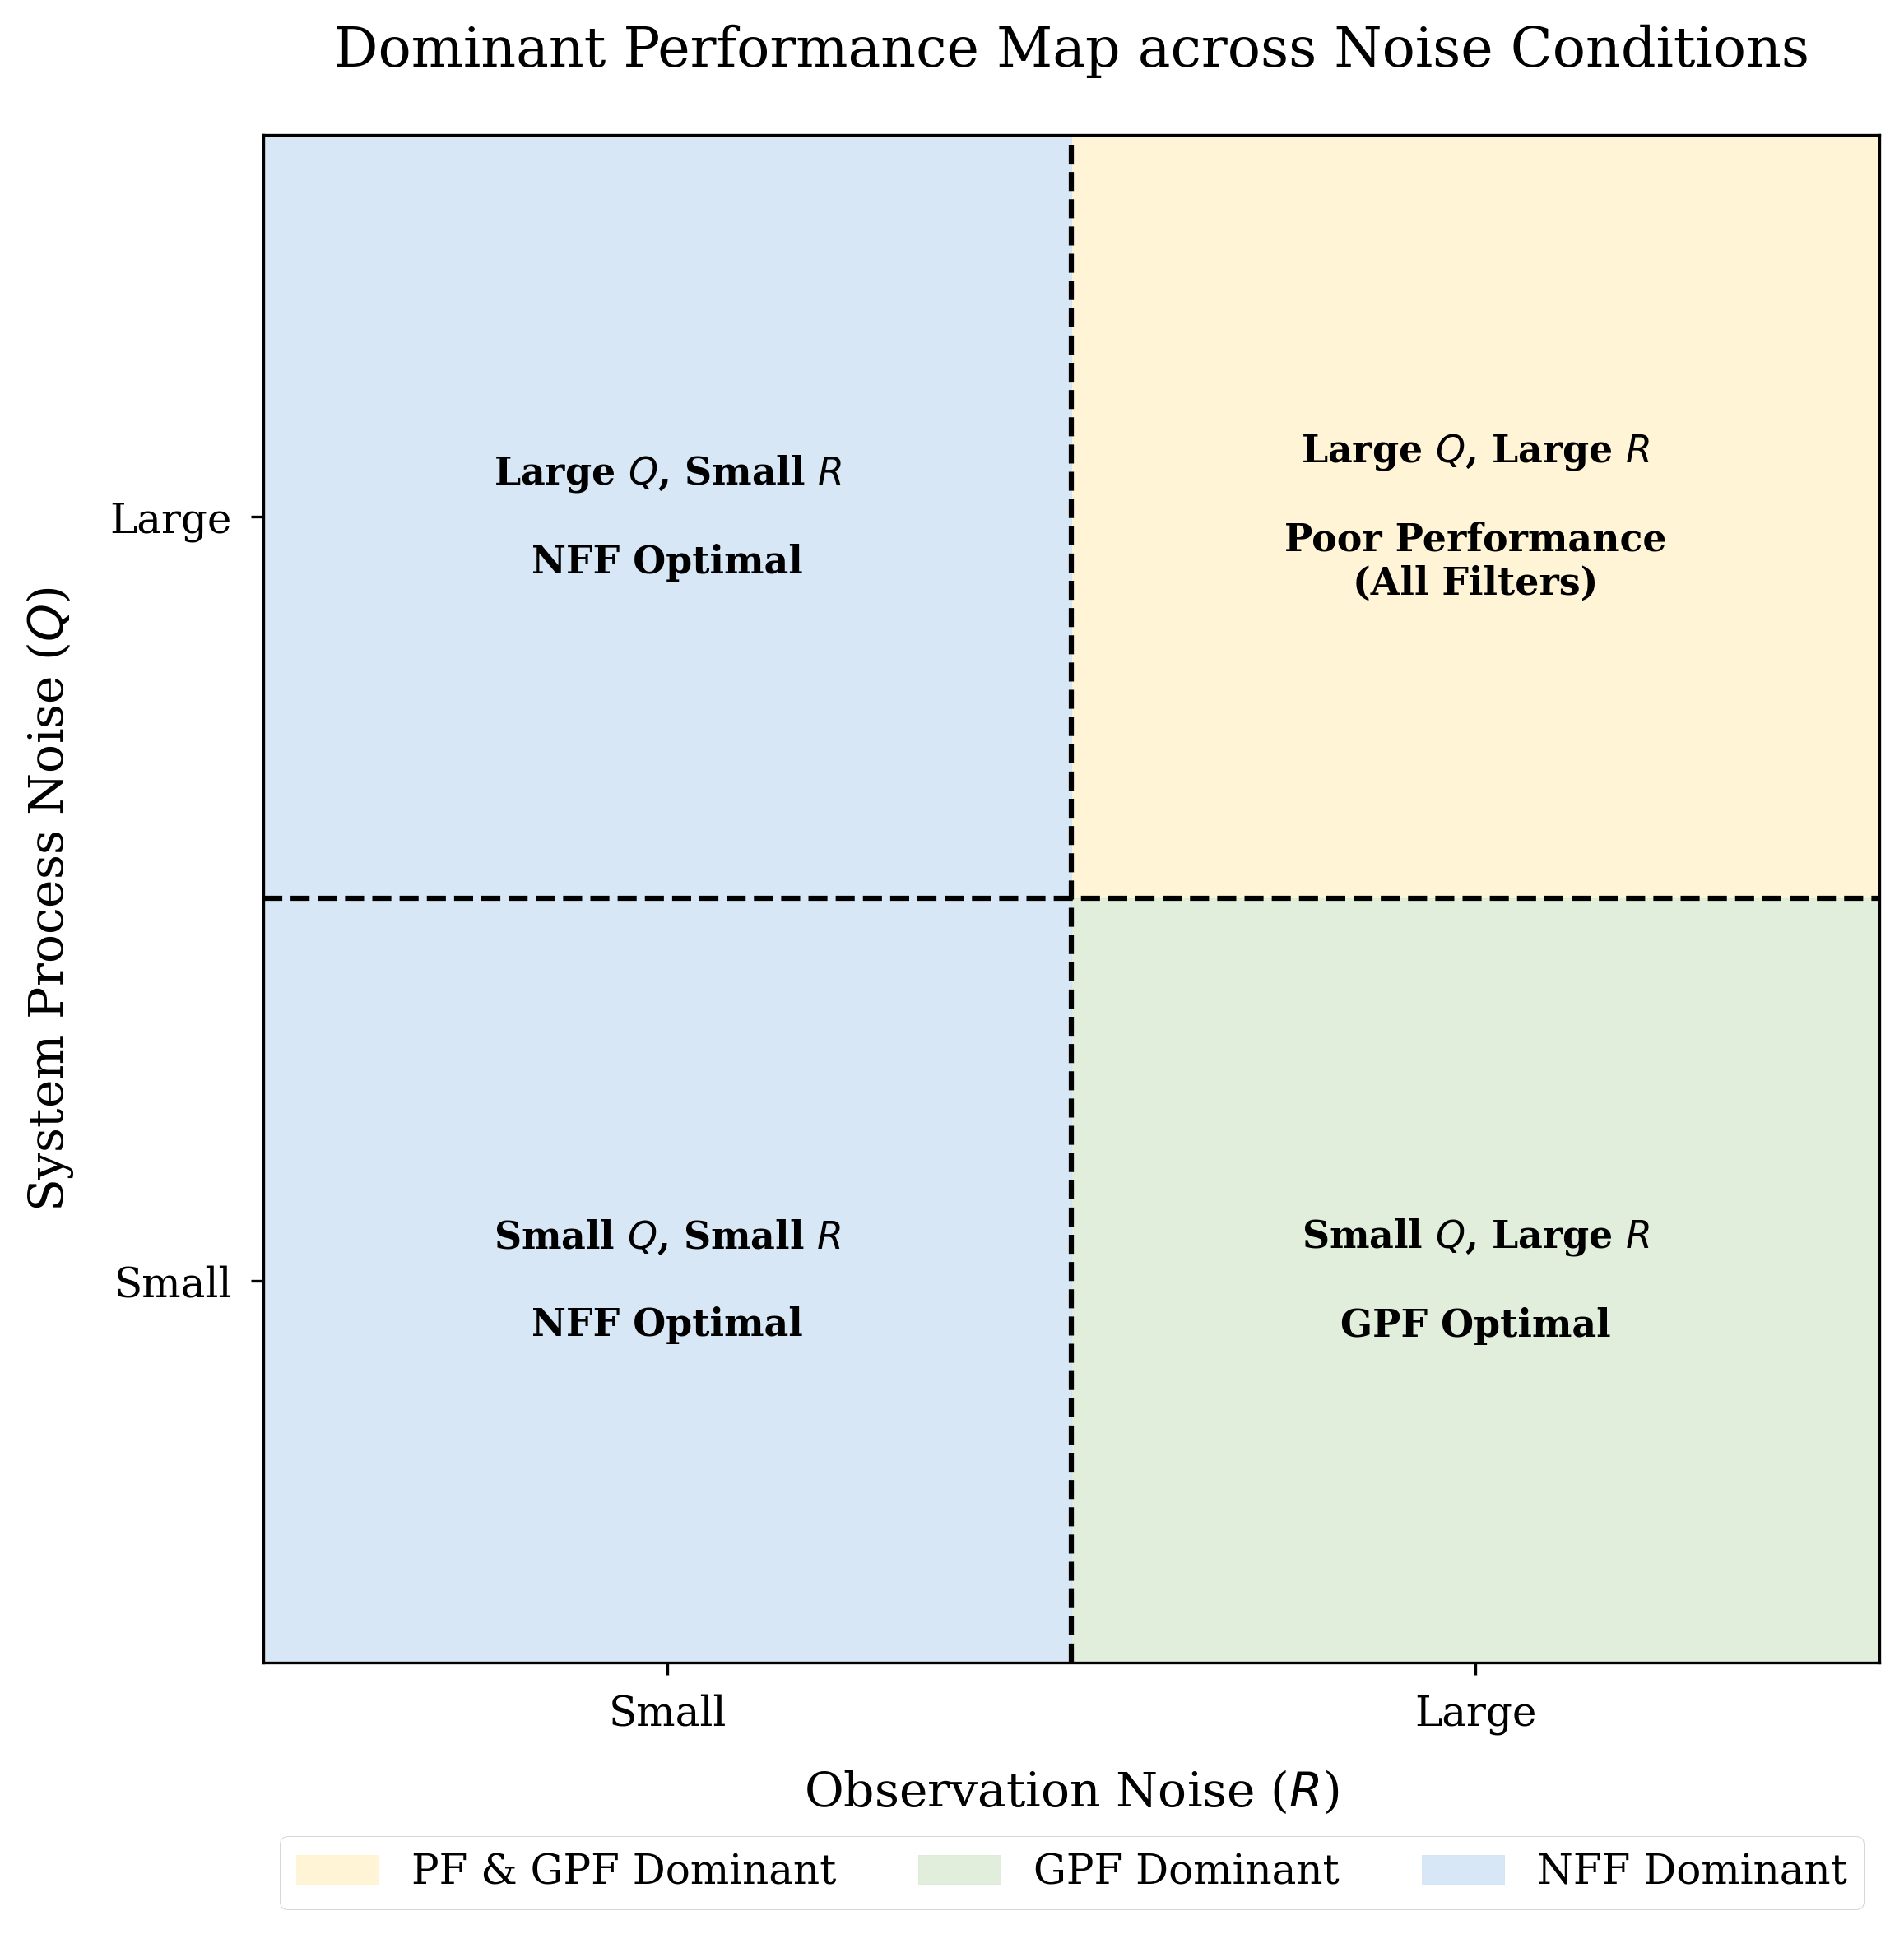
\includegraphics[width=0.9\textwidth]{figures/noise_quadrant.png}
    \caption{Dominant performance map of filters across different combinations of system process noise $Q$ and observation noise $R$.}
    \label{fig:noise_quadrant}
\end{Figure}

\begin{Table}[ht]
	\caption{Performance under extreme combinations of $Q$ and $R$. Comparison between best PF/GPF and NFF ($L=1000$).}
	\label{tab:extreme_noise_v2}
	\footnotesize
	\setlength{\tabcolsep}{5pt}
	\begin{tabular}{|c|l|c|c|cc|cc|}
		\hline
		& & & & \multicolumn{2}{c|}{NFF (C)} & \multicolumn{2}{c|}{NFF (NC)} \\ \cline{5-8}
		Condition & Metric & Best PF & Best GPF & M3 & M1 & M3 & M1 \\ \hline
		
		{Large $Q$ \& Large $R$} 
		& RMSE  & 5.668 & \textbf{5.644} & 5.662 & 5.793 & 5.793 & 5.875 \\
		& GAE   & 5.221 & \textbf{5.209} & 5.241 & 5.354 & 5.325 & 5.382 \\
		& MERF  & 0.567 & \textbf{0.565} & 0.567 & 0.581 & 0.581 & 0.589 \\
		& ANEES & \textbf{1.228} & 1.238 & 1.322 & 1.471 & 1.517 & 1.596 \\ \hline
		
		{Small $Q$ \& Large $R$} 
		& RMSE  & 12.007 & \textbf{3.715} & 5.036 & 5.043 & 7.097 & 6.926 \\
		& GAE   & 9.501  & \textbf{3.114} & 4.136 & 4.029 & 5.366 & 5.228 \\
		& MERF  & 1.201  & \textbf{0.372} & 0.505 & 0.505 & 0.711 & 0.694 \\
		& ANEES & NaN    & \textbf{3.306} & 41.513 & 43.444 & 51.552 & 82.882 \\ \hline
		
		{Small $Q$ \& Small $R$} 
		& RMSE  & 0.513 & 0.482 & \textbf{0.305} & 0.322 & 0.336 & 0.336 \\
		& GAE   & 0.469 & 0.407 & \textbf{0.283} & 0.295 & 0.309 & 0.309 \\
		& MERF  & 1.610 & 1.526 & \textbf{0.968} & 1.022 & 1.064 & 1.064 \\
		& ANEES & NaN   & NaN   & \textbf{4.222} & 5.464 & 5.958 & 6.241 \\ \hline
		
		{Large $Q$ \& Small $R$} 
		& RMSE  & 1.351 & 1.671 & 0.421 & 0.549 & \textbf{0.405} & 0.516 \\
		& GAE   & 1.271 & 1.550 & 0.362 & 0.479 & \textbf{0.349} & 0.449 \\
		& MERF  & 4.272 & 5.283 & 1.324 & 1.728 & \textbf{1.275} & 1.624 \\
		& ANEES & NaN   & NaN   & \textbf{2.837} & 7.936 & 3.362 & 7.667 \\ \hline
	\end{tabular}
\end{Table}

\clearpage